% Chapter 1

\chapter{Technological Foundation and Related Work} % Main chapter title

\label{chap_tech} % For referencing the chapter elsewhere, use \ref{Chapter1} 

This chapter will go over some research fields related to the topic of this thesis and aims to provide foundational knowledge that is useful to better understand the remainder of this thesis.
Section \ref{sec:genrl} contains information on the very basics of reinforcement learning, commonly used technologies, how to model a reinforcement learning problem, and how to solve it in a general manner. Most of the information and formulae in that chapter are derived from David Silver's course on reinforcement learning \citep{dsilver}.
Afterwards section \ref{sec:deeprl} will discuss how neural networks are a very important tool for the solving of reinforcement learning problems and some of the more specific networks that have proven useful.
Sections \ref{sec:a3ctheory} and \ref{sec:acktrtheory} will then discuss two of the specific algorithms, that were employed in this thesis and the sections at the end of this chapter depict some of the work that has already been done with StarCraft and StarCraft II in the context of artificial intelligence.
%----------------------------------------------------------------------------------------
\section{General Reinforcement Learning}
\label{sec:genrl}
\subsection{Markov Decision Process}
All reinforcement learning problems can be more or less be modelled as a Markov Decision Process (MDP). MDPs build the foundation of all reinforcement learning concepts and a lot of their terminology also stems from MDPs, which is the reason this section is going to introduce them.

While first thought of by Russian mathematician Andrei Andrejewitsch Markow, the earliest scientific paper about MDPs is "A Markovian Decision Process" by Richard Bellman \cite{Bel}. A Markov Decision Process is a mathematical representation of decision making problems and is an extension to Markov Processes and Markov Reward Processes.
\newpage
In essence a MDP is a tuple made up of five components:
\begin{itemize}
\item $S$ A finite set of states
\item $A$ A finite set of actions
\item $P$ A Transitionmatrix that contains the probabilities of transitioning from any state $s$ to any successor state $s'$ by taking action $a$
\item $R$ A Reward function
\item $\gamma$ The discount Factor
\end{itemize}

In an environment that is described by such a tuple an actor or agent chooses a number of consecutive actions. Each action results in a new state and gains the agent a reward specified by the reward function. The goal of the agent is to choose actions in a way that result in the maximum reward possible. 

Important for a MDP is, that all states in $S$ have the Markov Property. Having the Markov Property means that an individual state is memoryless and contains all the information needed in order to calculate the transition
$$s \xrightarrow[\text{a  }]{ } s'$$
without the need to know the history of which states were visited before. This requirement is not absolute however, but if it is not fulfilled a generalization of the MDP has to be applied, the partially observable markov decision process (POMDP) \citep{DBLP:journals/ai/KaelblingLC98,DBLP:journals/ior/SmallwoodS73}. These POMDPs observe the state of the underlying MDP not directly, but instead work with partial observations of the state, which, using a probability distribution, infer the actual state.  

Although the set of available states for the MDP is assumed to be finite, the resulting chain of choosing actions and transitioning to different states can become infinite. If it is, there is no maximum reward and the reward can become theoretically infinite as well. However, if there is a state $s$ that terminates the MDP then no actions can be chosen in this state and should the agent arrive in this state one episode is over and an end of episode reward is granted. 

The way the agent chooses it's actions is defined by a policy $\pi$, which is a probability function over actions given states, with
$$\pi(a|s)=\mathbb{P}[A_t = a | S_t = s]$$
This in turn means that to solve an MDP one needs to find the optimal policy $\pi_*$ that results in the highest reward from any given starting state. In order to find this policy one additional concept is needed: state- and action-value functions.
The state-value function of an MDP represents the expected reward of state $s$ while following policy $\pi$:
$$v_\pi(s) = \mathbb{E}_\pi[G_t | S_t = s ]$$
with $G_t$ being the reward that can be expected at the end of the entire episode, when starting at state $s$.
The action-value function is similar, giving the expected reward of taking action $a$ while in state $s$ and afterwards following policy $\pi$:
$$q_\pi(s, a) = \mathbb{E}_\pi[G_t | S_t = s, A_t = a ]$$
Knowing the action value function of an MDP for example, finding the optimal policy would be trivial. The optimal policy would simply be to always choose the most rewarding action $a$ for the current state $s$.
For simple MDPs these value functions can be represented by matrices with each cell representing the expected value of on state or state,action pair. 

To calculate these value functions, the expected reward $G_t$ needs to be determined. This can be done using the Bellman expectation equation. The Bellman equation splits the total reward $G_t$ into the immediate reward plus the discounted expected reward of all successive states/actions and defines the state and action value functions recursively:
$$v_\pi(s) = \mathbb{E}_\pi[R_t + \gamma \cdot v_\pi(S_{t+1}) | S_t = s]$$
$$q_\pi(s, a) = \mathbb{E}_\pi[R_t + \gamma \cdot q_\pi(S_{t+1}), A_{t+1} | S_t = s, A_t = a]$$
The Bellman expectation equation represents the value for a single policy. 
In order to find the optimal policy the Bellman optimality equation can be utilized. 
The optimality equation maximizes over all expectation equations.
$$v_*(s)= max_\pi v_\pi(s)$$
$$q_*(s, a) = max_\pi q_\pi(s, a)$$

\subsection{Solving MDPs}

\subsubsection{Policy Iteration / Actor-Only Methods}
\label{sec:pollearning}
One way to solve the Bellman optimality equation is through policy iteration. Policy iteration works through the use of two distinct steps: policy evaluation and policy improvement, which are applied in an alternating manner starting with the evaluation of a random policy.

A policy can be evaluated by estimating the value function in respect to the policy using the Bellman expectation equation.
$$v_\pi(s) = \mathbb{E}[R_{t+1} + \gamma R_{t+2} + ... | S_t = s]$$
This evaluation does not have to be calculated for the entire value function in each evaluation step, and can instead be approximated by sampling episodes from the environment by letting the agent take actions according to its current policy.

The actual evaluation of these samples can be done multiple ways, one of the more popular being the Monte-Carlo evaluation \citep{DBLP:conf/wsc/CerdaF97}. In Monte-Carlo evaluation only a single state, the starting state, has it's evaluation updated, and only after the entire episode is over. 

The other, more widely used method today is Temporal Difference(TD)-Learning \citep{DBLP:journals/ml/Sutton88}. In contrast to Monte-Carlo Learning, TD-Learning learns from incomplete episodes by approximating the expected reward using a backwards, or forwards view of n steps from the evaluated state. This results in a much more efficient and gradual evaluation by evaluation every single step and also makes it possible to learn MDPs that do not terminate. 


After sampling enough episodes for reaching an adequately accurate evaluation a new and improved policy is then gained by greedily updating according to the value function.
$$\pi'(s) = argmax_{\substack{a \in A}} Q(s,a)$$
It can be proven, that this policy update for simple problems almost always leads to the optimal policy even if the evaluation is only approximated with TD-Learning. This means the MDP can be solved, by alternating these evaluation and improvement steps until the policy is sufficiently stable.

The advantages of learning a policy directly are, that stochastic policies can be learned in addition to deterministic ones, and that policy algorithms tend to converge faster than value based ones. On the other hand they sometimes only converge to local optimums and not global ones and the policy evaluation is usually high variance. Being able to learn stochastic policies is especially important, as some problems cannot be solved in a deterministic manner.

Some notable examples for Actor-Only reinforcement learning methods are the REINFORCE algorithm \citep{DBLP:journals/ml/Williams92} and SRV \citep{DBLP:journals/nn/Gullapalli90}.

\subsubsection{Value Iteration / Critic-Only Methods}
\label{sec:vallearning}
Value iteration methods like SARSA\citep{Rummery94on-lineq-learning} and Q-Learning \citep{DBLP:journals/ml/WatkinsD92}, in contrast to policy iteration, never utilize an explicit policy. Instead, the value function itself is directly, iteratively improved according to Bellman's Optimality Equation.

Essentially this makes use of the fact, that a policy $\pi$ achieves the optimal reward from a state $s$ if, and only if, for any state $s'$ reachable from state $s$ $\pi$ also reaches the optimal reward. The resulting policy is in essence recursively split into two components: 
\begin{enumerate}
\item Taking the optimal action $a$ from state $s$
\item Taking the best action in respect to the optimal policy afterwards
\end{enumerate}

The Value update can be described by 
$$V_{i+1}(s) = max_a \sum_{s',r} P(s', r | s, a) [r + \gamma* V_i(s')]$$

For value iteration this update is all that is needed, and it can be applied iteratively until the difference between $V_{i}$ and $V_{i+1}$ is sufficiently small.
The actual policy is only derived when needed, by applying an $argmax$ across all states of the value function. In contrast to policy iteration methods this policy is strictly deterministic however.

\subsubsection{Q-Learning and Deep Q Networks}
Before the advent of A3C and other, newer reinforcement learning methods Q-Learning \citep{DBLP:journals/ml/WatkinsD92} and Deep Q-Networks(DQN)\citep{DBLP:journals/nature/MnihKSRVBGRFOPB15} in particular were among the most popular and well performing algorithms available. For this reason, and although they are neither used in this project nor are directly related, it was felt that they deserve a section in this chapter. 

Q-Learning is a value iteration method and attempts to learn the action-value function $Q(s, a)$ specifically. Actions in Q-Learning can then  be chosen in varying ways, for example using an $\epsilon-greedy$ strategy. 

In each step of the environment $Q(s, a)$ is improved iteratively by a small amount by applying the Bellman optimality equation. For small problems, where the $Q$ function can be represented by a matrix the update can be described as:
$$
Q(s, a) = r + \alpha *\gamma * max Q(s',a')
$$
$\alpha$ being the learning rate or step size, that determines how coarse the update steps are.

For more difficult problems however the $Q$ function is represented by a neural network instead, leading to Deep Q-Learning and DQN. The training is then done using backpropagation and a loss function, that attempts to minimize the mean squared error between the currently predicted $Q$ values and the actual target values that were obtained by taking the next action in the environment.
This iteration of taking actions and improving the network is repeated indefinitely and it can be shown, that this always converges somewhere close to the optimal value function.

DQN's are further characterized among other things by the many extensions that have been made to the core algorithm over time, that have been so powerful that they have become a staple for most implementations. Among these are "Experience Replay" \citep{DBLP:journals/corr/abs-1712-01275}, Double Q-Learning \citep{DBLP:conf/aaai/HasseltGS16} and "Dueling Networks"\citep{DBLP:journals/corr/WangFL15}. Experience Replay is a technique to feed the training samples obtained during training back into the network more than once, which stabilizes the network considerably. With Double Q-Learning not only one value function, but two and each sample updates one of those two value functions randomly. This in large prevents the overestimation of action values that are common in DQNs. Dueling Networks is not a modification to the algorithm itself. but  a specific neural network architecture following a similar idea as Double Q-Learning.


\subsubsection{Actor-Critic Methods}
\label{sec:accritic}
While most of the reinforcement learning algorithms used to fall into the categories of actor-only or critic-only methods described in \ref{sec:pollearning} and \ref{sec:vallearning} respectively, today Actor-Critic Methods are among the most popular reinforcement learning approaches.

Actor-Critic methods attempt to combine the main advantages of value based and policy based approaches. They try to both estimate the value function and estimate the policy at the same time.
They do this by implementing Generalized Policy Iteration, meaning that they also alternate between a policy evaluation and a policy improvement step.

The critic part is responsible for evaluating the value function, that the policy implemented by the actor is based on. The actual evaluation can be done a number of ways, for example TD-Learning, and always relies on taking samples from the environment.

The actor's policy is not directly inferred from the value function however, but updated only in small steps. In which direction the policy parameters should be updated is given by the policy gradient as estimated by for example, finite differences \citep{DBLP:journals/technometrics/Hesterberg04} or likelihood ratios \citep{DBLP:journals/cacm/Glynn90}. These small updates along the policy gradient lead to smoother conversion and reduce oscillation. 

The updated policy is then used by the actor to choose and take an action in the environment, which 
results in a new sample, that can used in the next evaluation step.

\section{Deep Reinforcement Learning}
\label{sec:deeprl}
Up until now, state-, and action-value functions were represented as tabular matrices for simplicities' sake. For most interesting applications this does not work however, as state- and action-spaces are simply too large to fully solve iteratively. Since these value functions are arbitrary functions though, they can also be approximated using function approximators like linear combinations of features, nearest neighbour, decision trees or neural networks. 

Approximating the value functions enables an algorithm to extrapolate from seen states to unseen states and by that eliminates the need to learn each individual state. Instead of actual states, the algorithm can now learn a set of parameters $w$ of the value function with:
$$\hat{v} _\pi(s, w) \approx v_\pi(s) $$
$$\hat{q} _\pi(s, a, w) \approx q_\pi(s, a) $$
As with value iteration the actual policy can be simply inferred by acting greedily according to this now approximated value function.
The next section will describe one of the techniques for approximating a value function that is commonly used, Stochastic Gradient Descent. The following sections \ref{sec:cnn} and \ref{sec:lstm}
will then cover two specific neural network architectures, that have proven especially useful in reinforcement learning.

\subsection{Stochastic Gradient Descent}
\label{sec:sgd}
For stochastic gradient descent or SGD, if $J$ is any differentiable function, e.g. a neural network, then the gradient of $J$ can be defined as 
$$\bigtriangledown_wJ(w)=
\begin{pmatrix}
\frac{\partial J(w)}{\partial w_1} \\
\vdots
\frac{\partial J(w)}{\partial w_n}
\end{pmatrix}
$$

In order to find a minimum of this gradient the parameter vector $w$ has to be adjusted in the direction of the gradient.

$$ \Delta w = -\frac{1}{2}\alpha\bigtriangledown_wJ(w)$$

with $\alpha$ being a constant, that denotes how much the parameters $w$ are adjusted in each step.

For function approximation in reinforcement learning specifically, the goal is to minimise the mean squared error between the estimated function using parameter vector $w$ and the actual value function $v_\pi$. The actual value function is not known of course, as otherwise no reinforcement learning would be needed. Instead the value function at state $s$ is estimated by taking a sample from the environment. This sample is the (discounted) reward received after taking an action chosen by the current policy from state $s$. 


\subsection{CNN}
\label{sec:cnn}
\begin{figure}[htb]
  \centering
      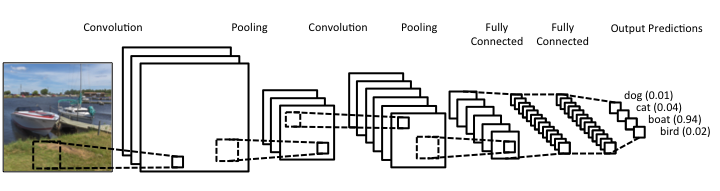
\includegraphics[width=1\textwidth]{Figures/cnn.png}
  \caption{ Overview over a sample Convolution Neural Network, From left to right the input image is processed by convolutional layers, pooling layers and last by fully connected layers, which output a prediction}
\end{figure}
Convolutional neural networks or CNNs are particularly important for deep reinforcement learning on video games. CNN's are what make it possible to directly use the rendering output of the game as the environment's observations. They are very similar to regular neural networks in that they still have interconnected layers with learned weights, have a loss function on the last fully connected layer, and still express a single differentiable function from input to output. The biggest difference to a regular neural network is that a CNN explicitly assumes that all inputs are images in the form of raw pixels, and has specific architecture to deal with them.

The original architecture for CNNs is the LeNet architecture \citep{leCun}, proposed in 1998. 
While there have been developed many new architectures since, like AlexNet\citep{alexnet}, GoogleNet \citep{googlenet}, or ResNet \citep{DBLP:journals/corr/HeZRS15}, which improve greatly on it's effectiveness, most of these architecture still make use of the same or at least similar building blocks to create the neural network.   
These components are

\begin{enumerate}
\item Convolution
\item Activation Function
\item Pooling
\item Fully Connected Layers
\end{enumerate}

During the convolution step a series of filters is applied to the image. In addition to the neuron weights, the convolution filter values are learned by the CNN as well. The size, number, and stride of these filters is specified before training though and can be treated as hyperparameters. After training each of these filters represents one feature, that has been learned by the network.
The activation function, most notably a linear Rectifier(RelU), is applied after each convolution step. This is done in order to bring non-linearity into an otherwise linear system. This is important, as the real world can rarely be described in completely linear terms.

Pooling Layers drastically reduce the size of the convolved images by grouping nearby pixels together and taking for example their maximum, minimum or average value as the pixel value for the resulting image. This increases training speed, but more importantly leads to translation invariance in regards to the input.

Components 1. till 3. can be chained together multiple times before flattening their output into a single feature vector and then following up with one or multiple fully connected layers. These fully connected layers can either be normal neural network layers or more specialized layers like for example RNN layers or the LSTM layers described in the following section.


\subsection{Long Short-Term Memory Networks}
\label{sec:lstm}
LSTM units \citep{lstm,DBLP:journals/neco/GersSC00} are a form of recurrent neural network layer, that is especially adept at discerning temporal dependencies between subsequent inputs. Since temporal dependencies tend to be quite important when interacting with an environment like in reinforcement learning, LSTM layers can be an excellent choice for function approximation. 

Nevertheless, they require the training samples generated by the reinforcement learning algorithms to be processed in the correct temporal order. As the A3C algorithm is an inherently asynchronous algorithm, that can not guarantee the order in which the samples are added to the training queue, LSTMs were not used in this project. While the ACKTR and A2C algorithms are synchronous, and the A2C algorithm even comes with an optional LSTM policy, this policy was not used and instead all of the algorithms use the same basic CNN policy. 

\section{Asynchronous Advantage Actor-Critic (A3C)}
\label{sec:a3ctheory}
\begin{figure}[htb]
  \centering
      \includegraphics[width=1\textwidth]{Figures/A3C_Overview.pdf}
  \caption{ Overview of the general A3C Architecture. Multiple workers interact with their own environments in parallel and trade their learned information with one global network }
  \label{fig:a3cover}
\end{figure}

The A3C algorithm is a somewhat recent reinforcement learning algorithm released by Google's DeepMind team \citep{DBLP:journals/corr/a3c}. It became very popular very fast, as it made Deep Q Networks, which were incredibly popular before, practically obsolete. It performs not only better and more robustly, but from own experience it is also easier to implement.

As the name implies it is an Actor-Critic reinforcement learning method as described in section \ref{sec:accritic}. But, instead of one actor-critic pair working on one environment, A3C makes use of multiple Workers, that each have their own Neural Network parameters and interact with their own environment as illustrated by Figure \ref{fig:a3cover}. The samples generated by these workers are then played back asynchronously into one global network. This is preferred over the single environment approach, because, in addition to the performance benefit of parallel processing, all of these Workers are independent from each other resulting in much more diverse samples.

This global network has one input, the current state $s$ and two distinct outputs: a softmax activated probability distribution $P$ over all actions $a$ acting as the policy 
$$\pi_\theta(s)$$
and an estimate of the value function for the input state.

The "Advantage" part of the algorithm's name comes from the use of the advantage value $A$ during the policy gradient step instead of the discounted reward $R$. The advantage estimate helps the agent to not only establish how good a given action is, but also how much better it turned out than expected.
The advantage value can be calculated using:
$$A = Q(s, a) - v(s)$$ 
As A3C does not approximate $Q(s, a)$ directly, it is replaced by the discounted reward $r$.
This reward $r$ is calculated as an n-step discounted return, utilizing a forward view. This means, that updates to the network parameters can not be applied immediately and instead have to be processed in batches in order to calculate this n-step return. While this introduces policy lag, this was found to be easier than using a backward view with eligibility traces in some cases.
For exploration purposes entropy should be added to policy $p$ as well, as otherwise a convergence to local minimums is likely. The loss function to be optimised therefore has 3 components and is defined as: 
$$L_{total} = L_{\pi} + L_{v} + L_{entropy}$$
The policy loss $L_{\pi}$ describes the total reward that an agent can achieve averaged over all starting states, and is calculated as
$$L_\pi = E[A(s, a) * log \pi(s, a)]$$
This is the expected advantage value over the probability distribution of policy $\pi$. For batch processing this policy loss is additionally averaged over all samples.

The value loss $L_v$ utilizes the fact, that the true value function is estimated in accordance with the Bellman Equation. 
$$V(s_0) = r_0 + \gamma r_1 + \gamma^2 r_2 + ... + \gamma^n V(s_n)$$
With an n-step return the loss is the difference, between the current estimation of rewards of a state, and the estimation after n steps.
$$L_v = r_0 + \gamma r_1 + \gamma^2 r_2 + ... + \gamma^n V(s_n) - V(s_0)$$
Again, this loss is averaged over all samples in a batch.

Maximizing the entropy pushes the policy away from a fully deterministic policy. The entropy for a single sample can be defined as
$$H(\pi(s)) = \sum\limits_{a} \pi(s)_a \cdot log \pi(s)_a$$
with $\pi(s)_a$ being the probability of taking action $a$ while in state $s$.
To get the  full $L_{entropy}$ one again averages over all samples and then negates the result, as the loss function is minimized and the entropy has to be maximized.
$$L_{entropy} = \sum\limits{i=1}^{k H(\pi(s_i))}$$

The optimization of this loss function could be done by Stochastic Gradient Descent as shown in section \ref{sec:sgd}, but RMSPROP \citep{rmsprop} has been shown to be the most robust \citep{DBLP:journals/corr/a3c}.

One slightly different version of the A3C algorithm is the A2C algorithm that was released in conjunction with the ACKTR algorithm by OpenAI\citep{openaiblog-a2c}. A2C is used for testing in this project as well and is closely related to the A3C algorithm. Essentially it is simply a synchronized variant of the same algorithm, hence the name "Advantage Actor-Critic". Tests done by the OpenAI team show, that the asynchronicity of A3C does not result in tangible performance benefits\citep{openaiblog-a2c}.

\section{Actor-Critic Kronecker-Factored Trust Region (ACKTR)}
\label{sec:acktrtheory}
ACKTR, proposed by a group of researchers from both University of Toronto and New York University in late 2017\citep{DBLP:journals/corr/abs-1708-05144} is an even more advanced and state of the art algorithm than A3C. The authors posit, that sample efficiency is the primary metric of concern for reinforcement learning algorithms. In both simulated and even more so real world environments getting training samples and stepping through the environment is much slower than the actual processing of the algorithm. For that reason the authors propose an algorithm that manages to learn complex problems much faster than other algorithms with being around 25\% slower to compute but being much more sample efficient.

Most reinforcement learning algorithms use relatively simplistic optimization techniques like stochastic gradient descent, that are rather inefficient. ACKTR however aims to utilize more sophisticated optimization strategies, while employing and combining ideas from multiple different reinforcement learning algorithms.

Similar to A3C and A2C algorithms for example ACKTR is an actor-critic algorithm that uses multiple environment workers to reduce training time and increase sample diversity. Yet, the optimization is an extension of the optimization of the natural policy gradient algorithm.

The problem with the natural policy gradient is, that the natural gradient can not be directly computed and has to be estimated. Trust Region Policy Optimization(TRPO) \citep{DBLP:journals/corr/SchulmanLMJA15} is one of the algorithms that does that, but TRPO is sample inefficient and does not lend itself to be used with large models.

The key idea of the ACKTR algorithm is to calculate this gradient by using Kronecker-factored approximated curvature(K-FAC)\citep{DBLP:journals/corr/MartensG15}.
Gradient updates using K-FAC only take marginally longer to compute than an SGD update, but utilizing a natural gradient makes this algorithm much more sample efficient.

\section{Reinforcement Learning in StarCraft}
The primary paper building the basis for this thesis is StarCraft II: A New Challenge for Reinforcement Learning \citep{DBLP:journals/corr/dmsc2}. This paper introduces the PySC2 framework and offers evaluations for basic scenarios that were gained using some of DeepMinds own Neural Networks. These scenarios are largely abstract and very simple however, and do not reflect the actual competitive game of StarCraft II. This thesis aims to improve that aspect.

DeepMind implemented the A3c algorithm either using the AtariNet, which DeepMind used to successfully learn a multitude of Atari Games or FullyConvNet, a fully convolutional Neural Net with no fully connected layers but optionally with LSTM layers. 

As both PySC2 and the StarCraft II Machine Learning API have been released there are only very few scientific articles that make use of them. There are however a considerable amount of papers on StarCraft II's predecessor, StarCraft: Broodwar. It's API, while not officially endorsed by Blizzard has been around for many years and has gathered a sizeable community.

While papers on StarCraft: Broodwar are not fully applicable to StarCraft II there are considerable similarities in the gameplay of these two games, making these papers at least somewhat related. 
Among these papers is \citep{broodwarRL}, which is the namesake of this thesis and the paper the idea for this thesis comes from. This paper explores the StarCraft:Broodwar API at the example of one small combat scenario utilizing Q-Learning and SARSA algorithms and evaluates their suitable in that context. It was able to achieve decent success in that specific scenario through the usage of highly abstracted actions, and a very limited action and observation space. The scenario in question is further discussed in section \ref{sec:failed}.

A very similar topic, unit micro-management, is discussed in the paper \citep{scai:unitmicro}, and a more general view on combat in Real-Time-Strategy(RTS) games can be found in \citep{scai:gamecombat}. There are also a considerable amount of papers on other aspects of StarCraft reinforcement learning, that do not directly relate to combat scenarios. \citep{scai:bo} for example concerns itself with the planning of build orders for optimal economic growth.

\section{Non RL StarCraft AI(Bots)}
Before reinforcement learning became relevant for StarCraft AI there was already a sizeable community around writing regular AI bots. While they are only peripherally related, they can give insights to interesting scenarios and problems for StarCraft Bots, while also being a useful benchmark. \\Although not available in the form of scientific articles, the most popular hard-coded bots are automaton 2000 and Ursadak. Both of these Bots leverage tens of thousands of actions per minute as their main advantage. Automaton 2000 for example executes approximately 100 actions per minute(APM) per single unit that it controls. No human, and likely also no reinforcement algorithm can come close to that number, especially with larger unit groups. Sometimes they even employ borderline cheating for even more impressive results. Figure \ref{fig:aut} shows an example of that. 

\begin{figure}[htb]
  \centering
      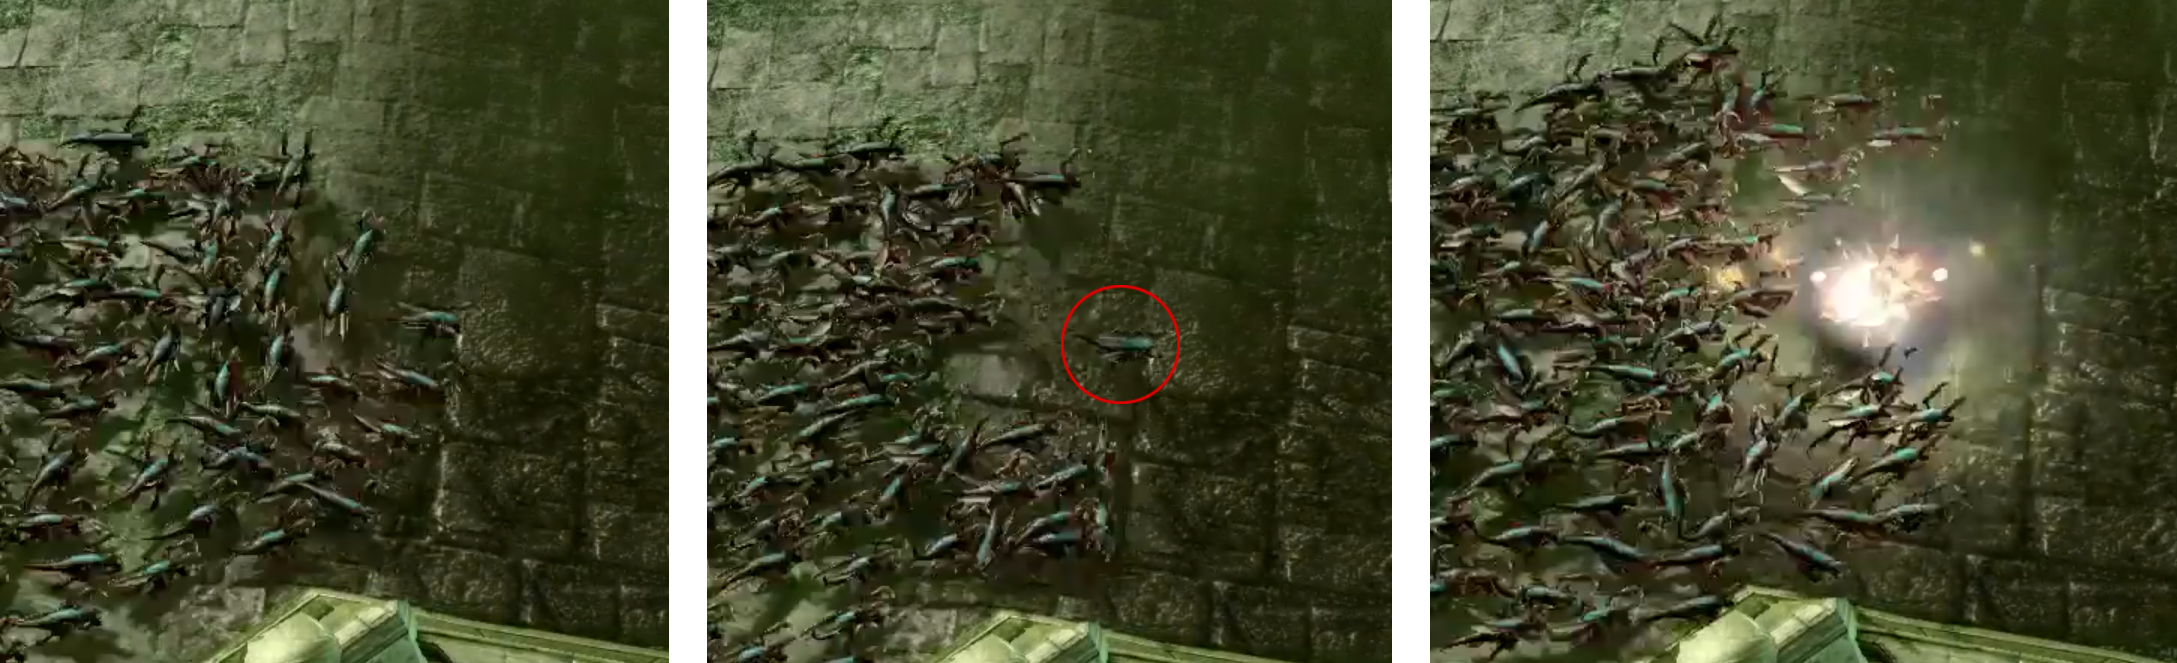
\includegraphics[width=1\textwidth]{Figures/aut2000.png}
  \caption{ Example of advanced techniques used by microbot AUtomaton 2000. With knowledge of which unit an area of effect attack is going to land it can split its army in order to minimize the damage incurred.}
 \label{fig:aut}
\end{figure}

Automaton manages to figure out which of its units is targeted next by enemy fire, information that should not be available and at least is not available to human players. With its high APM it can use this information for pulling away units nearby the targeted unit in the event of an area of effect attack, thus preventing almost all damage of the attack. In the video this Figure is taken from, 100 Zerglings are pitted against 20 Tanks, tanks being AoE(Arrea of Effect) attacking units specifically designed for defeating large groups of Zerglings. In this test and without the microbot, all Zerglings are defeated without destroying more than 2 tanks. With microbot's active micromanagement however, all Tanks are defeated, after which about a dozen of Zerglings are still left alive. 

This shows how potent this combination of high APM and usually not available or hard to obtain information is. In contrast to Automaton 2000, Ursadak is not only a microbot, that concerns itself solely with the micromanagement of units, and instead is a fully featured bot, that is able to play the complete game of StarCraft II as the terran race. While there are many more bots and especially microbots for StarCraft II, these are 2 of the more popular ones, having been featured on prominent StarCraft II tournaments for showcasings. There even are full AI only tournaments where Bots battle each other either in specialized scenarios, or the actual games of StarCraft/StarCraft II \citep{scai:comps}.




